\documentclass[11pt]{article}

\usepackage[margin=1in]{geometry}
\usepackage[T1]{fontenc}
\usepackage[utf8]{inputenc}
\usepackage{lmodern}
\usepackage{microtype}
\usepackage{amsmath,amssymb}
\usepackage{booktabs}
\usepackage{tabularx}
\usepackage{graphicx}
\usepackage{float}
\usepackage{hyperref}
\usepackage{caption}
\usepackage{subcaption}
\usepackage{enumitem}
\usepackage{xcolor}

\hypersetup{colorlinks=true,linkcolor=blue,citecolor=blue,urlcolor=blue}
\graphicspath{{revised_report_assets/}{/mnt/data/revised_report_assets/}}

\newcommand{\ER}{G(n,d/n)}
\newcommand{\E}{\mathbb{E}}
\newcommand{\Prob}{\mathbb{P}}
\newcommand{\whp}{\text{w.h.p.}}
\newcommand{\dd}{\,\mathrm{d}}

\title{Integer Programming for Large Independent Sets\\in Sparse Random Networks and ca-GrQc Real Network}
\author{Keming Miao, Ziqian (Alice) Xiao, Bowen Yu}
\date{\today}

\begin{document}
\maketitle

\begin{abstract}
We study the maximum independent set problem on sparse Erdős--Rényi graphs
$G(n,d/n)$ and on the SNAP ca-GrQc collaboration network.  We are interested
not only in the size of the independent sets returned by a warm-started integer
program, but also in whether the solver certifies optimality.  On
$G(n,20/n)$, a multi-seed experiment over sizes $n=100$ through $5000$ shows
random-order greedy closely following the finite-$d$ prediction
$\log(1+d)n/d$, while minimum-degree greedy gives substantially larger warm
starts for CBC.  CBC certifies all $n=100$ random instances, but every larger
random instance in this experiment ends without a matching upper bound; for
$n\ge 500$, the final incumbent is just the minimum-degree warm start.  Thus,
on the larger random instances, the limiting issue is certification rather
than the construction of a large feasible set.
By contrast, on the real ca-GrQc network, connected-component decomposition
makes the same IP formulation effective as an exact method, allowing CBC to
\emph{certify} $\alpha(G)=2459$, while minimum-degree greedy returns 2458.  The contrast
suggests that the same IP formulation is limited less by vertex count alone
than by graph structure, with the sparse random graphs leaving CBC with weak
global certificates and ca-GrQc splitting into many components and containing
collaboration cliques that make exact certification tractable.
\end{abstract}

\section{Introduction}

The maximum independent set problem asks for the largest set of vertices in a
graph with no edges among the selected vertices.  In this project, we evaluate an
integer-programming formulation for this problem on two classes of sparse
graphs, namely Erdős--Rényi random graphs $G(n,d/n)$ \cite{erdosrenyi1959},
with particular attention to the case $d=20$, and the SNAP ca-GrQc
collaboration network, a real graph with clustering, heterogeneous degrees,
and many connected components.

The asymptotic scale of maximum independent sets in $G(n,d/n)$ is well known
\cite{coja2015}, with the independence number in the double asymptotic regime
$n\to\infty$ followed by $d\to\infty$ being on the order of
\[
\frac{2\log d}{d}n,
\]
whereas simple greedy procedures achieve only about
\[
\frac{\log d}{d}n.
\]
The question is therefore whether integer programming can meaningfully
\emph{exceed} the random-order greedy scale, and whether it can provide optimality
\emph{certificates} at the graph sizes considered here.

Our results separate the quality of feasible solutions from the ability to
prove optimality.  On the tested random graphs, the warm-started IP pipeline
returns feasible independent sets above the random-order greedy scale, but the
solver usually cannot prove that these incumbents are optimal.  In the
multi-seed random-graph experiment, CBC certifies optimality for all $n=100$
instances, but for $n\ge 200$ it terminates with a nonzero certificate gap.  On
ca-GrQc, after decomposing the graph into connected components, the IP
formulation instead certifies the exact value $\alpha(G)=2459$.

\section{IP Formulation}

For a graph $G=(V,E)$, an independent set is a subset $S\subseteq V$ such that
no two vertices in $S$ are adjacent.  The independence number is
\[
\alpha(G)=\max\{|S|: S\subseteq V,\; S\text{ independent}\}.
\]
The standard binary integer-programming formulation uses a variable
$x_v\in\{0,1\}$ for each vertex and solves
\[
\begin{aligned}
\max \quad & \sum_{v\in V}x_v\\
\text{s.t.}\quad & x_u+x_v\le 1, && (u,v)\in E,\\
& x_v\in\{0,1\}, && v\in V.
\end{aligned}
\]
The edge constraints ensure that adjacent vertices cannot both be selected, so
the feasible binary vectors are precisely the incidence vectors of independent
sets.

In the computations we solve the equivalent minimum vertex-cover formulation.
With the change of variables $y_v=1-x_v$, the model becomes
\[
\begin{aligned}
\min \quad & \sum_{v\in V}y_v\\
\text{s.t.}\quad & y_u+y_v\ge 1, && (u,v)\in E,\\
& y_v\in\{0,1\}, && v\in V.
\end{aligned}
\]
If $\tau(G)$ denotes the minimum vertex-cover value, then
\[
\alpha(G)=|V|-\tau(G).
\]
In our computations, CBC was more stable on this cover formulation once warm starts
were enabled.

For instances that are not solved to optimality, we report both incumbent
quality and the remaining certificate gap.  Let $L$ denote the best feasible
independent set size found by the solver.  In the vertex-cover formulation,
CBC also maintains a lower bound $B_{\mathrm{VC}}$ on the optimal cover size,
which gives the independent-set upper bound
\[
U=|V|-\lceil B_{\mathrm{VC}}\rceil.
\]
Thus
\[
\alpha(G)\in[L,U].
\]
We also record the warm-start size $W$ and the improvement
\[
\Delta=L-W.
\]
The value of $\Delta$ is a useful diagnostic because it indicates whether CBC actually
improved on the greedy solution used to initialize the solve.

\section{Theory Benchmarks}

The leading asymptotic expression $2\log(d)n/d$ gives the correct scale when
$d$ is large, but it is not a sharp numerical prediction at $d=20$, so we
compare the experiments against the random-order greedy prediction and a
first-moment upper benchmark as two finite-$d$ reference quantities.

\subsection{Greedy Scale}

Consider random-order greedy, which processes vertices in a uniformly random
order and accepts a vertex whenever it has no previously accepted neighbor.
Let $s(t)$ denote the accepted fraction after a fraction $t$ of vertices has
been processed.  For $G(n,d/n)$, a standard differential-equation calculation
in the style of Wormald's method for random graph processes \cite{wormald1995}
gives
\[
\frac{\dd s}{\dd t}=\exp(-d s(t)),\qquad s(0)=0.
\]
A newly exposed vertex is accepted when it has no edge into the
already accepted set, whose size is approximately $s(t)n$.  Solving the
differential equation yields
\[
s(t)=\frac{\log(1+dt)}{d},
\qquad
s(1)=\frac{\log(1+d)}{d}.
\]
For $d=20$,
\[
\frac{\log(21)}{20}=0.1522,
\]
which is close to the threshold
\[
\frac{\log(20)}{20}=0.1498.
\]
Accordingly, $\log(1+d)n/d$ and $\log(d)n/d$ are both useful benchmarks for
the greedy scale in our experiments.

\subsection{First-Moment Upper Benchmark}

A finite-$d$ first-moment calculation provides a sharper upper reference than
the leading large-$d$ expression.  Let $N_k$ be the number of independent sets
of size $k=an$.  Then
\[
\E[N_k]=\binom{n}{k}(1-d/n)^{\binom{k}{2}}.
\]
By Stirling's formula,
\[
\frac{1}{n}\log \E[N_{an}]
=
H(a)-\frac{d a^2}{2}+o(1),
\]
where
\[
H(a)=-a\log a-(1-a)\log(1-a).
\]
If
\[
H(a)-\frac{d a^2}{2}<0,
\]
then Markov's inequality rules out independent sets of size $an$ with high
probability.  Thus the largest positive root of
\[
H(a)-\frac{d a^2}{2}=0
\]
serves as a finite-$d$ upper benchmark.  At $d=20$, this root is
\[
a_{\mathrm{FM}}=0.232996.
\]
This is substantially below
\[
\frac{2\log(20)}{20}=0.2996,
\]
so the first-moment benchmark is the more informative reference for the
moderate-degree experiments reported below.

\section{Implementation}

We implemented and compared three procedures.

\begin{itemize}[leftmargin=*]
\item \textbf{Random-order greedy} processes vertices in random order and
accepts each vertex whenever possible.  We used 20 random permutations in the
low-time-limit comparison and 100 random permutations per instance in the
multi-seed random-graph experiment.
\item \textbf{Minimum-degree greedy} selects a vertex of current minimum
degree at each step, after which the selected vertex together with its neighbors is
removed from the graph.
\item \textbf{IP/CBC} solves the binary vertex-cover formulation in
PuLP 3.3.0 using CBC 2.10.3, initialized with the best greedy solution
available \cite{forrestcbc}.
\end{itemize}

For each Erdős--Rényi instance, we generated a graph from $G(n,20/n)$, ran the
greedy baselines, used the best greedy solution as a warm start, and then
solved the vertex-cover IP subject to the stated time limit.  The main random
graph experiment uses 20 seeds each for $n=100,200,500,1000$, 10 seeds each
for $n=1500,2000,3000$, and 5 seeds for $n=5000$, with a 300-second CBC limit
for $n\le 1000$ and a 600-second limit for the larger scaling sizes.  We also
use a single-seed low-time-limit comparison, with limits of 30 seconds at
$n=100$, 20 seconds for
$200\le n\le 2000$, and 60 seconds at $n=3000$.  For each run we recorded the
warm-start size $W$, final incumbent $L$, improvement $\Delta=L-W$, converted
upper bound $U$, and whether CBC certified optimality.

For the ca-GrQc experiment, we first converted the SNAP edge list into a simple
undirected graph by symmetrizing duplicate directed rows, removing self-loops,
and retaining vertices that became isolated after loop removal, then split the
resulting graph into connected components.  Since independence number is
additive over connected components,
\[
\alpha(G)=\sum_i \alpha(G_i),
\]
we solved the IP separately on each component and summed the resulting optima.

We also included clique inequalities in the random-graph IP computations.  In the
independent-set variables, every clique $C$ yields
\[
\sum_{v\in C}x_v\le 1.
\]
In the vertex-cover variables $y_v=1-x_v$, this becomes
\[
\sum_{v\in C}y_v\ge |C|-1.
\]
We used triangle and 4-clique cuts for the random graphs.  These cuts were not
used for ca-GrQc; after component decomposition, the edge formulation was
already sufficient for the real-network instance.

All returned independent sets were verified directly against the edge list.
As a separate sanity check, small validation instances were solved both by CBC
and by exhaustive search.  The two methods agreed on
\[
(n,d,\alpha)=(12,3,6),\quad (14,4,5),\quad (16,5,7).
\]
All experiments were run on an Apple M3 Pro with 18 GB RAM, Python 3.9.6,
PuLP 3.3.0, and CBC 2.10.3.  The notebook and supporting code are available in
the project repository \cite{code}.

\section{Random Graph Experiments}

For the Erdős--Rényi part of the project, we use the completed multi-seed
experiment as the main source of evidence rather than relying on a single
random seed.  It uses 20 seeds each for $n=100,200,500,1000$, 10 seeds each
for $n=1500,2000,3000$, and 5 seeds for $n=5000$.  Within each instance,
random-order greedy is averaged over 100 permutations, the best of
random-order greedy and minimum-degree greedy is used as the IP warm start,
and CBC is then asked both to improve the incumbent and to prove an upper
bound.  We used a 300-second limit for $n\le 1000$ and a 600-second limit for
the larger scaling sizes.

\begin{table}[H]
\centering
\caption{Multi-seed summary for $G(n,20/n)$.  Ratios are means over seeds.
Here $L$ is the incumbent independent-set size and $U$ is CBC's converted upper
bound on $\alpha(G)$.  The certified and uncertified columns count how many
instances did or did not receive an optimality certificate.}
\label{tab:er-long}
\scriptsize
\setlength{\tabcolsep}{4pt}
\begin{tabular}{rrrrrrrrr}
\toprule
$n$ & graphs & certified & uncertified & rand./$n$ & min-deg/$n$ & $L/n$ & $U/n$ & time/graph \\
\midrule
100  & 20 & 20 & 0  & 0.1442 & 0.1830 & 0.1990 & 0.1990 & 14.3s \\
200  & 20 & 0  & 20 & 0.1485 & 0.1888 & 0.1963 & 0.2513 & 300.6s \\
500  & 20 & 0  & 20 & 0.1508 & 0.1924 & 0.1924 & 0.3219 & 290.7s \\
1000 & 20 & 0  & 20 & 0.1515 & 0.1931 & 0.1931 & 0.3552 & 161.2s \\
1500 & 10 & 0  & 10 & 0.1515 & 0.1955 & 0.1955 & 0.3678 & 599.6s \\
2000 & 10 & 0  & 10 & 0.1519 & 0.1965 & 0.1965 & 0.3760 & 596.9s \\
3000 & 10 & 0  & 10 & 0.1521 & 0.1953 & 0.1953 & 0.4000 & 403.5s \\
5000 & 5  & 0  & 5  & 0.1522 & 0.1958 & 0.1958 & 0.4293 & 596.3s \\
\bottomrule
\end{tabular}
\end{table}

\begin{figure}[H]
\centering
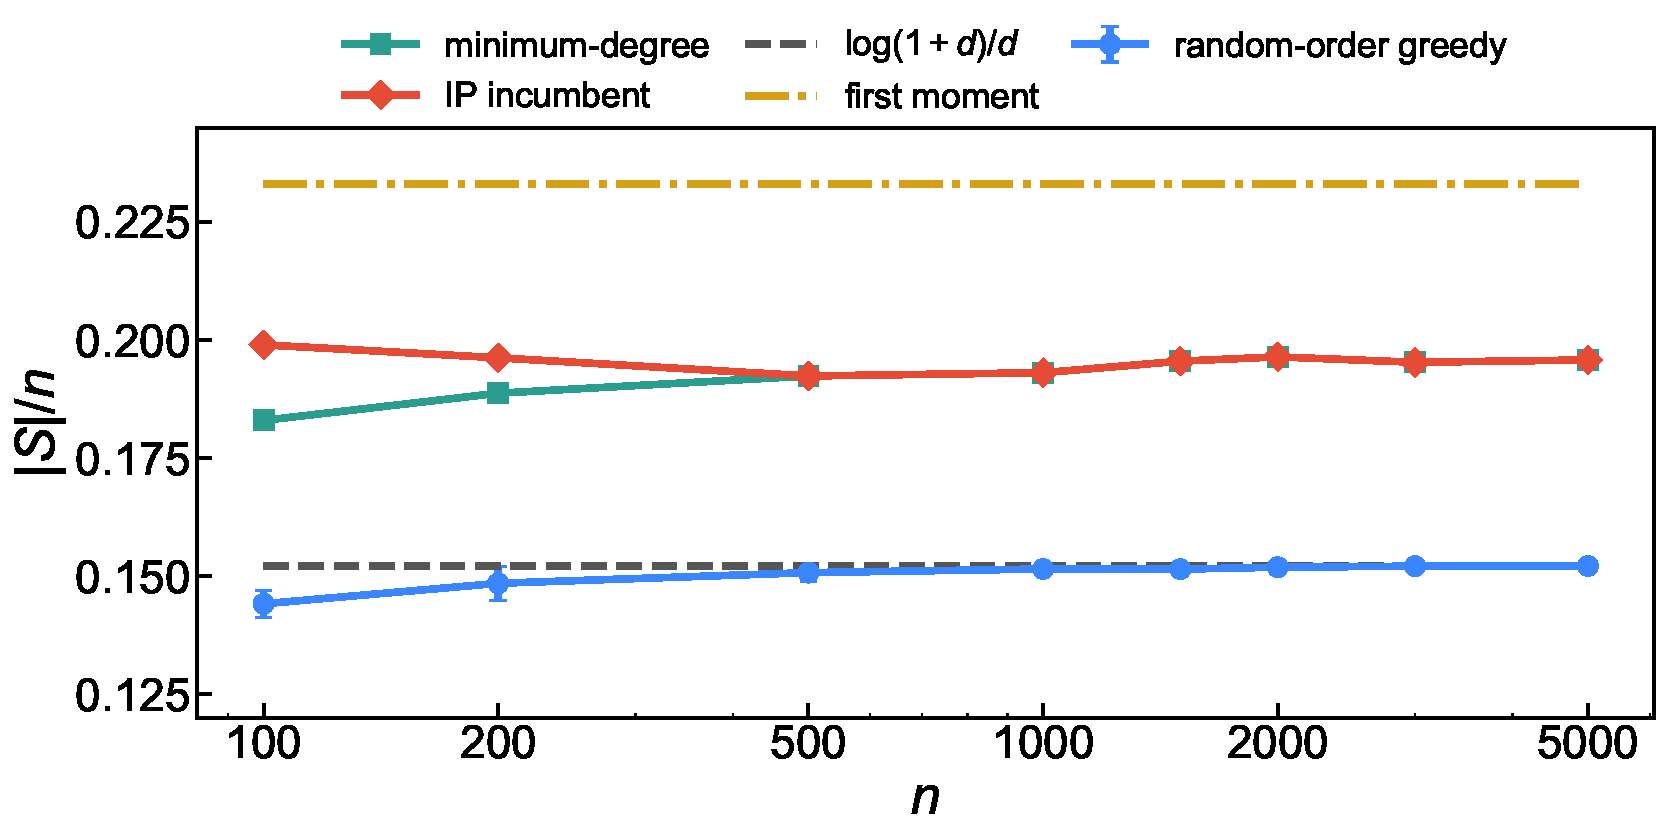
\includegraphics[width=0.85\linewidth]{results/figure5_long_batch_ratios.pdf}
\caption{Feasible independent-set sizes found on $G(n,20/n)$, normalized by
$n$ and averaged over seeds.  Random-order greedy is the basic baseline,
minimum-degree greedy is the warm start given to CBC, and the IP curve is
CBC's best feasible set at termination, with certification shown separately in
Figure~\ref{fig:er-time-gap} and the CBC incumbent coinciding with the
minimum-degree warm start from $n\ge 500$.}
\label{fig:er-long-ratios}
\end{figure}

\begin{figure}[H]
\centering
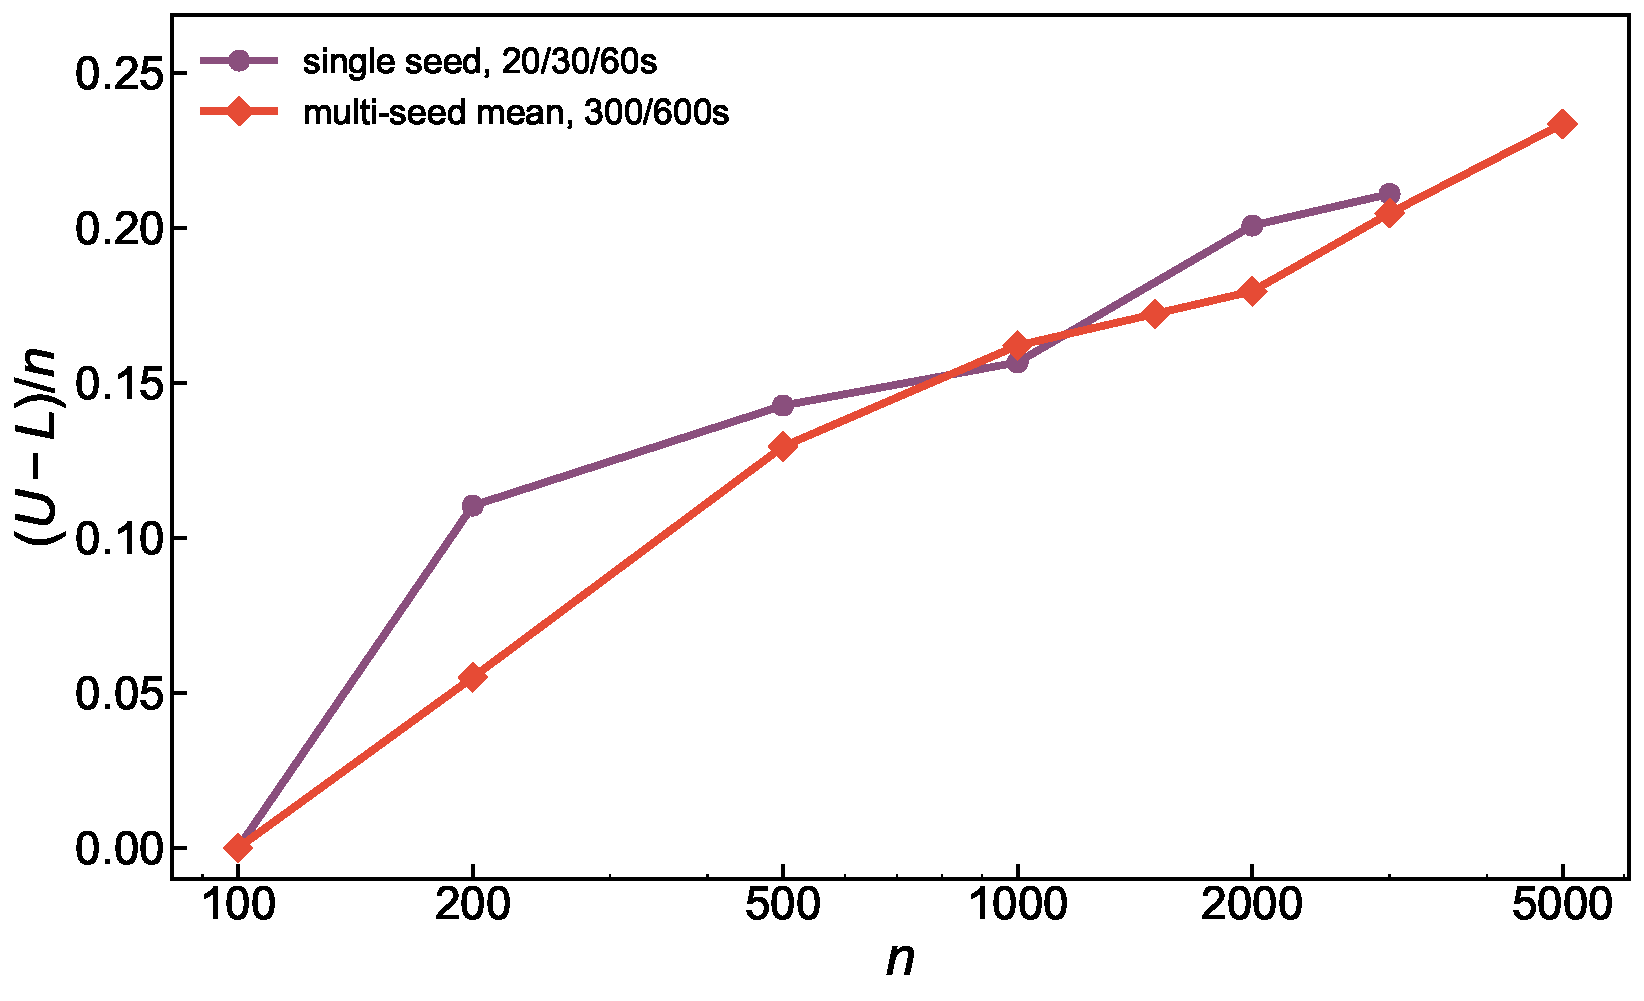
\includegraphics[width=0.82\linewidth]{results/figure7_time_limit_gap_comparison.pdf}
\caption{Certificate gap comparison between a single-seed random-graph
experiment with 20/30/60-second limits and a multi-seed random-graph
experiment with 300/600-second limits.  The larger time budget reduces the gap
for several sizes, while the larger random graphs still end with nonzero
certificate gap.}
\label{fig:er-time-gap}
\end{figure}

The random-order greedy results agree closely with the finite-$d$ greedy
prediction, with mean density rising from $0.1442$ at $n=100$ to $0.1522$ at
$n=5000$, essentially the value of $\log(1+20)/20$.  Minimum-degree greedy is
consistently larger, around $0.19$--$0.20$ over the tested sizes, while CBC
sometimes improves the warm start by a few vertices at $n=200$ but still does
not certify optimality.  From $n=500$ onward, the recorded incumbent in the
multi-seed experiment equals the warm start in every run.

Within the given time limit, the larger random graphs remain uncertified, as
illustrated by the multi-seed experiment at $n=3000$, where the mean incumbent
density is $0.1953$ and the mean converted upper-bound density is $0.4000$.
The shorter-and-longer time-limit comparison in
Figure~\ref{fig:er-time-gap} shows that giving CBC more time closes part of the
certificate gap, especially at the smaller sizes, while the gap remains
nonzero on the larger random graphs.  The random-graph experiment therefore separates the task of
quickly obtaining a large feasible independent set through minimum-degree
greedy from the harder task of closing the optimality gap with CBC at these
sizes.

\section{Real Network Experiment on SNAP ca-GrQc}

We further implement the real-network instance on the SNAP ca-GrQc collaboration graph
\cite{leskovec2007snap,snapca}.  It records coauthorship in the arXiv General
Relativity and Quantum Cosmology category; a paper with $k$ authors contributes
a $k$-clique to the graph.  SNAP reports 5242 nodes and 14496 raw edges.  After
symmetrizing duplicate rows, removing self-loops, and retaining vertices that
become isolated after loop removal, our simple graph has
\[
n=5242,\qquad m=14484,\qquad \bar d=\frac{2m}{n}=5.526.
\]
The graph has 355 connected components, with the largest component containing
4158 vertices.  We solve the IP separately on each component and sum the
component optima.

\begin{table}[h]
\centering
\caption{SNAP ca-GrQc independent set results.}
\label{tab:snap}
\begin{tabular}{lr}
\toprule
quantity & value \\
\midrule
random greedy mean, 20 permutations & 2179.20 \\
random greedy standard deviation & 15.17 \\
random greedy best, 20 permutations & 2202 \\
minimum-degree greedy & 2458 \\
IP optimum & 2459 \\
IP certificate & exact \\
total IP time & 35.1 seconds \\
\bottomrule
\end{tabular}
\end{table}

\begin{figure}[h]
\centering
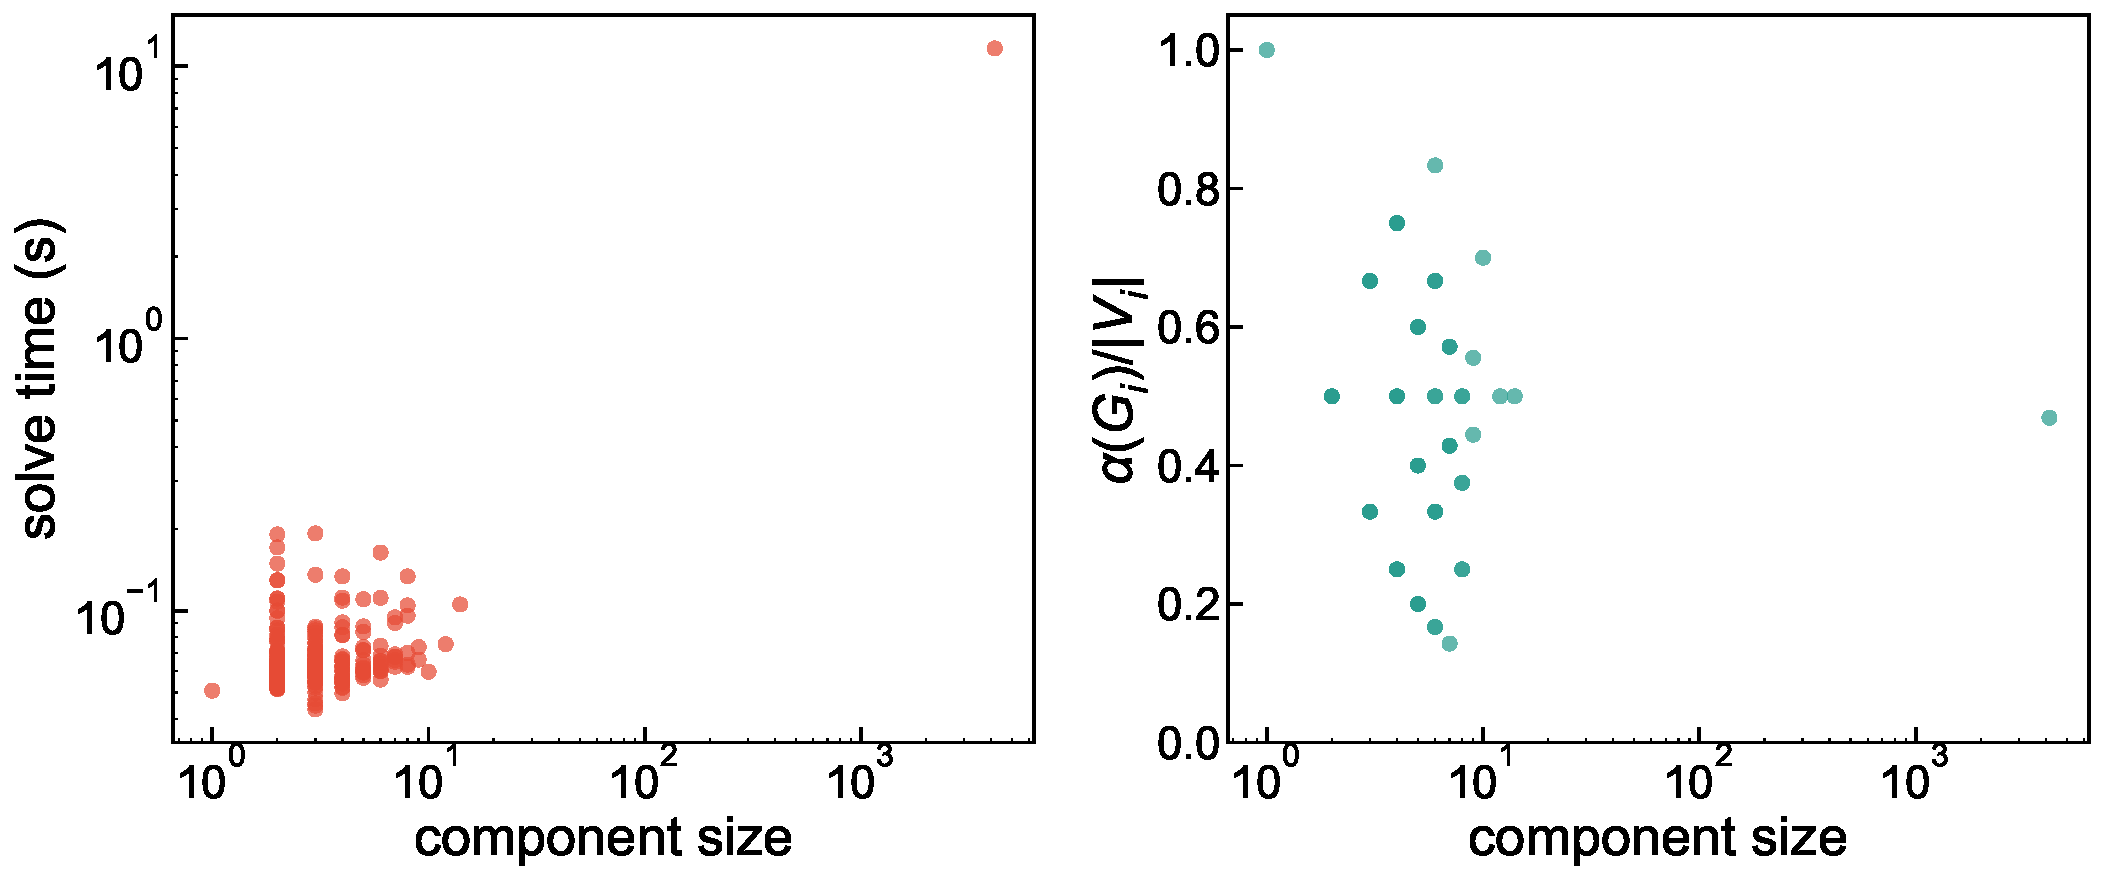
\includegraphics[width=0.94\linewidth]{results/figure4_snap_component_profile.pdf}
\caption{Component-level profile for ca-GrQc.  The largest component is the
dominant subproblem in solve time, while the smaller components contribute
little computational cost and often have high independent-set density.}
\label{fig:snap-components}
\end{figure}

The component-wise IP solve certifies
\[
\alpha(G_{\mathrm{ca\text{-}GrQc}})=2459.
\]
Minimum-degree greedy obtains 2458, which is
\[
\frac{2458}{2459}=99.96\%
\]
of the certified optimum.  Random-order greedy is substantially weaker, with
average performance
\[
\frac{2179.20}{2459}=88.62\%
\]
of the optimum over 20 random permutations.

Substituting the observed average degree $\bar d$ into the Erdős--Rényi
benchmarks gives
\[
\frac{\log \bar d}{\bar d}n=1621.6,\qquad
\frac{\log(1+\bar d)}{\bar d}n=1779.4,
\]
\[
a_{\mathrm{FM}}n=2625.5,\qquad
\frac{2\log \bar d}{\bar d}n=3243.2.
\]
The certified optimum lies above the greedy-scale predictions and below the
finite-$d$ first-moment upper benchmark, although this comparison is only a
null-model reference because the structural features of ca-GrQc differ
significantly from those of an Erdős--Rényi graph with the same average degree.

\begin{table}[h]
\centering
\caption{ca-GrQc and one matched Erdős--Rényi null instance generated with the
same $n$ and expected average degree $\bar d$.}
\label{tab:matched}
\scriptsize
\setlength{\tabcolsep}{4pt}
\begin{tabular}{lrrrrrrlr}
\toprule
graph & $n$ & $m$ & comps. & rand. mean & min-deg & $L$ & $U$ & time \\
\midrule
ca-GrQc & 5242 & 14484 & 355 & 2179.20 & 2458 & 2459 & 2459 & 35.1s \\
matched ER & 5242 & 14782 & -- & 1763.15 & 2115 & 2115 & 2605 & 32.1s \\
\bottomrule
\end{tabular}
\end{table}

The matched Erdős--Rényi control uses $p=\bar d/n$.  On this control instance,
after the same 30-second budget, CBC has incumbent 2115 and converted upper
bound 2605.  The ca-GrQc instance, in contrast, is solved exactly after
component decomposition. Therefore, this comparison establishes a narrow structural point that the
advantage comes from the particular component structure and collaboration
geometry of ca-GrQc, rather than from vertex count or density alone.

\section{Discussion}

The sparse random graph experiments highlight the distinction between
incumbent quality and proof of optimality, since the primal side of the
computation is strong enough for minimum-degree greedy to quickly find feasible
independent sets above the random-order greedy scale, while the dual side is
much weaker and leaves CBC with large upper-bound gaps on the larger
$G(n,20/n)$ instances even though, in branch-and-bound terms, the solver is
initialized with a good incumbent.

As Figure~\ref{fig:er-time-gap} shows, CBC improves the warm start on the
smallest random instances and sometimes improves it at $n=200$, although no
$n=200$ run is certified, and for $n\ge 500$ the multi-seed records show zero
improvement over the warm start, so the empirical gain over random-order greedy
at those sizes comes from the minimum-degree initialization.

The ca-GrQc experiment demonstrates a different use of the same IP formulation,
where the graph's 355 connected components reduce one 5242-vertex problem to
many smaller subproblems and, together with the structure of the coauthorship
network, make exact certification feasible.  In this setting, the IP
formulation is useful not only for storing a strong incumbent but also for
proving optimality.

The comparison with random-graph formulas requires some care because, at
$d=20$, the first-moment benchmark is around $0.233n$, whereas the leading
large-$d$ expression $2\log(d)n/d$ is around $0.300n$.  For the random
instances, the observed incumbents fall between the random-order greedy scale
and this finite-$d$ first-moment benchmark, while for the real network the
Erdős--Rényi quantities are best viewed as baselines rather than predictions
because ca-GrQc is far from an Erdős--Rényi graph.

\section{Conclusion}

On $G(n,20/n)$, the warm-started IP pipeline returns feasible independent sets
larger than the random-order greedy scale across the completed multi-seed
experiment, although this success comes mostly from the minimum-degree greedy
warm start.  CBC certifies all $n=100$ instances, but for $n\ge 200$ it does not certify
optimality within the time limit, and for $n\ge 500$ it does not improve the
warm start, so on the larger sparse random graphs the IP approach does not
solve the problem in the exact optimization sense.

On the SNAP ca-GrQc collaboration network, the same formulation performs much
better after connected-component decomposition, with CBC certifying
\[
\alpha(G)=2459,
\]
while minimum-degree greedy obtains 2458 and random-order greedy averages
2179.20.  The real-network experiment shows that IP can provide exact
certificates on structured sparse networks even when it struggles to close
optimality gaps on sparse Erdős--Rényi instances of comparable size.

Overall, random-order greedy matches the expected $\log(1+d)n/d$ scale on the
random graphs, minimum-degree greedy is substantially stronger, and IP is most
valuable when it can convert a strong incumbent into a proof of optimality.  In
our experiments, that certification succeeds on ca-GrQc but not on the larger
tested Erdős--Rényi graphs.

\section*{Acknowledgments}

We thank Professor David Gamarnik for all the great lectures and for his guidance on this project. We also acknoledge the use of AI tools (ChatGPT 5.5) for proofreading and editing the report, but all the scientific content and analysis were done by the authors.

\begin{thebibliography}{9}

\bibitem{erdosrenyi1959}
P. Erdős and A. Rényi.
\newblock On random graphs. I.
\newblock \emph{Publicationes Mathematicae}, 6:290--297, 1959.

\bibitem{coja2015}
A. Coja-Oghlan and C. Efthymiou.
\newblock On independent sets in random graphs.
\newblock \emph{Random Structures \& Algorithms}, 47:436--486, 2015.

\bibitem{wormald1995}
N. C. Wormald.
\newblock Differential equations for random processes and random graphs.
\newblock \emph{Annals of Applied Probability}, 5(4):1217--1235, 1995.

\bibitem{forrestcbc}
J. Forrest and the CBC team.
\newblock CBC User Guide.
\newblock COIN-OR Branch-and-Cut solver documentation,
\url{https://www.coin-or.org/Cbc/cbcuserguide.html}.

\bibitem{leskovec2007snap}
J. Leskovec, J. Kleinberg, and C. Faloutsos.
\newblock Graph evolution: Densification and shrinking diameters.
\newblock \emph{ACM Transactions on Knowledge Discovery from Data}, 1(1):2,
2007.

\bibitem{snapca}
Stanford Network Analysis Project.
\newblock General Relativity and Quantum Cosmology collaboration network.
\newblock \url{https://snap.stanford.edu/data/ca-GrQc.html}.

\bibitem{code}
B. Yu, K. Miao, A. Xiao.
\newblock 18.619 Final project code and notebook.
\newblock \url{https://github.com/bowenyu066/18.619-final-project}.

\end{thebibliography}

\end{document}
